\subsection{Contractual Refinement}
The simplest restructuring that could be done on the model was to split any guarantees containing an $\land$ at the highest level of the binary Boolean statement and create additional guarantees from this split. For instance, if GUARANTEE0 = A and B, then split this into GUARANTEE1 = A, GUARANTEE2 = B. This provided an easy way to test that our assumption was correct regarding the types of minimal cut sets generated given various forms of contracts. Algorithm~\ref{alg:splitAnd} shows this process. 

\begin{algorithm}[h]
\SetKwFunction{FMain}{$splitOnAnd$}
 \SetKwProg{Fn}{Function}{:}{}

	\Fn{\FMain{expression}}{
		Program $P$ \;
		Guarantees $list_G$ \;
		\For{all $g \in list_G$}{
			\If{binary statement with operator $\land$}{
			    insert into $P$ $\rightarrow$ new guarantee (left) \;
			    insert into $P$ $\rightarrow$ new guarantee (right) \;
				splitOnAnd(left) \;
				splitOnAnd(right) \;
			} %end if there exists AND in G
		}%end for all g in P
	}
	\caption{Split guarantees on logical AND operator}
	\label{alg:splitAnd}
\end{algorithm}

The sensor encoded into Lustre originally has a single guarantee as shown in Figure~\ref{fig:lustreOneGuar} and the results of Algorithm~\ref{alg:splitAnd} can be seen in Figure~\ref{fig:lustreTwoGuar}. 

\begin{figure}[h!]
\begin{center}
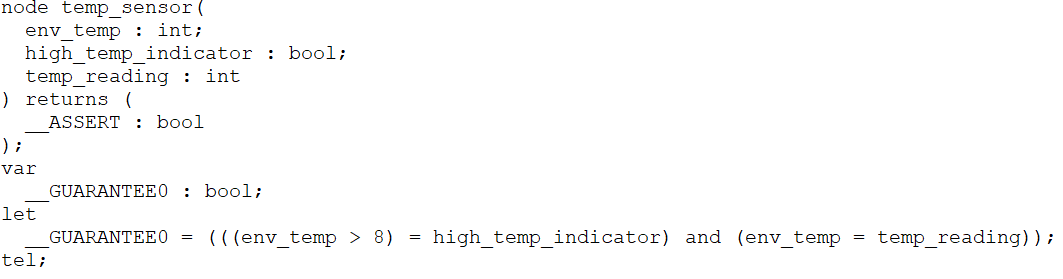
\includegraphics[width=1.0\textwidth]{images/lustreTwoGuar.PNG}
\caption{Temp Sensor With Original Guarantee} \label{fig:lustreOneGuar}
\end{center}
\end{figure} 

\begin{figure}[h!]
\begin{center}
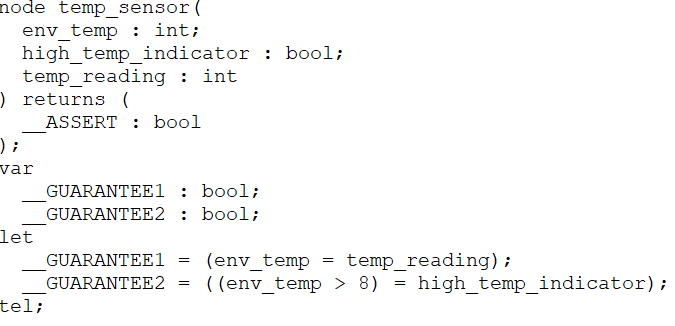
\includegraphics[width=.8\textwidth]{images/lustreOneGuar.PNG}
\caption{Temp Sensor With Modified Guarantees} \label{fig:lustreTwoGuar}
\end{center}
\end{figure} 

Given the property \texttt{((env\_temp $>$ 8) $=$ sensor\_high)}, in the first case, \texttt{GUARANTEE0} is the IVC. In the second case, only \texttt{GUARANTEE2} is the IVC for the property. The minimal cut sets produced reflected what we expected and show two faults in the cut set for Figure~\ref{fig:lustreOneGuar} and only the high temp indicator fault for the analysis in Figure~\ref{fig:lustreTwoGuar}. 

While this algorithm is efficient and quite simple, it only catches the low hanging fruit, so to speak. Due to the logical nature of how the Lustre model is analyzed, all guarantees are viewed as a conjunction; therefore, splitting guarantees into new statements only works on the $\land$ operator. This is sufficient for illustration and an initial test into the problem, but insufficient for full analysis of the issue. 

\danielle{Do some timing results to compare IVC generation and fault analysis with unmodified versions of projects. Put in results section?}